\noindent The indicator $\mathbf{1}\{y \le z\}$ in Eq.~1 jumps from 0 to 1 at $z = y$. The integrand is the squared distance between the forecast CDF and a hard step function at the observation.

\paragraph{Strict propriety.}
A scoring rule $S(F, y)$ is strictly proper if, for any $F$ and any true distribution $G$,
%
\begin{equation}
    \mathbb{E}_{y \sim G}\bigl[ S(F, y) \bigr] \ge \mathbb{E}_{y \sim G}\bigl[ S(G, y) \bigr],
\end{equation}
%
with equality if and only if $F = G$ almost surely. \citet{gneiting2007strictly} prove that CRPS satisfies this property: a forecaster who reports the true distribution scores best in expectation.

\paragraph{The implicit assumption.}
The propriety theorem treats $y$ as a draw from $G$. It says nothing about the relationship between $y$ and the underlying physical or social quantity that $G$ describes. The CRPS formula treats the reported $y$ \emph{as if} it were the true value: the indicator function has no width.

For some data sources this is correct. A coin flip outcome is exact. A digital weather station's temperature has measurement uncertainty small relative to forecast uncertainty, so treating the reading as exact is harmless. But for other data sources it is not. Conflict fatality counts come from coding pipelines that aggregate media reports, witness accounts, and expert judgement. The UCDP Georeferenced Event Dataset \citep{ucdp_codebook} explicitly provides low/best/high estimates per event and documents systematic underreporting in remote regions. The reported best estimate is a noisy summary of an underlying truth---and similar observation uncertainty arises in disease surveillance \citep{gibbons2014measuring} and other domains where data are compiled from heterogeneous sources.

\paragraph{Why the assumption matters.}
When the assumption is violated, CRPS systematically rewards narrow, overconfident forecast distributions over wider, more honest ones that better represent the underlying uncertainty. Concretely: if UCDP records 12 deaths in a cell-month but the true count is plausibly between 8 and 30, a forecast that says ``exactly 12'' scores better under classical CRPS than one that spreads probability across that range---even though the wider forecast better represents what is actually known. I quantify this bias in \S6.

The existing literature includes one well-known modification in this direction: threshold- and quantile-weighted CRPS \citep{gneiting2011comparing}, which rescales the integrand to emphasise specific regions of the distribution. This addresses a different problem---the Forecaster's Dilemma \citep{lerch2017forecasters}, in which conditioning forecast evaluation on extreme observations systematically discredits skillful forecasts. In conflict forecasting, this means that evaluating models only on high-fatality months rewards models that predict high fatalities uniformly; weighted scoring rules are a complementary, not competing, tool. Crucially, weighted CRPS does not lift the assumption that the observation is known precisely. The reformulation I propose is orthogonal: it modifies the indicator function rather than the weight on the integrand.

\paragraph{Visual illustration.}
Figure~\ref{fig:step_vs_sigmoid} illustrates the CDF comparison underlying classical CRPS (left) and the reformulated metric (right) for the same forecast and the same observed value. In the classical version, $F_\text{obs}$ is a step at $y$, and the area between $F_\text{pred}$ and $F_\text{obs}$ is large unless $F_\text{pred}$ is very narrow. In the reformulated version, $F_\text{obs}$ is a smooth CDF reflecting observational uncertainty, and the area is smaller for the same forecast, because the forecast is no longer asked to match an impossibly precise step.

\begin{figure}[h]
    \centering
    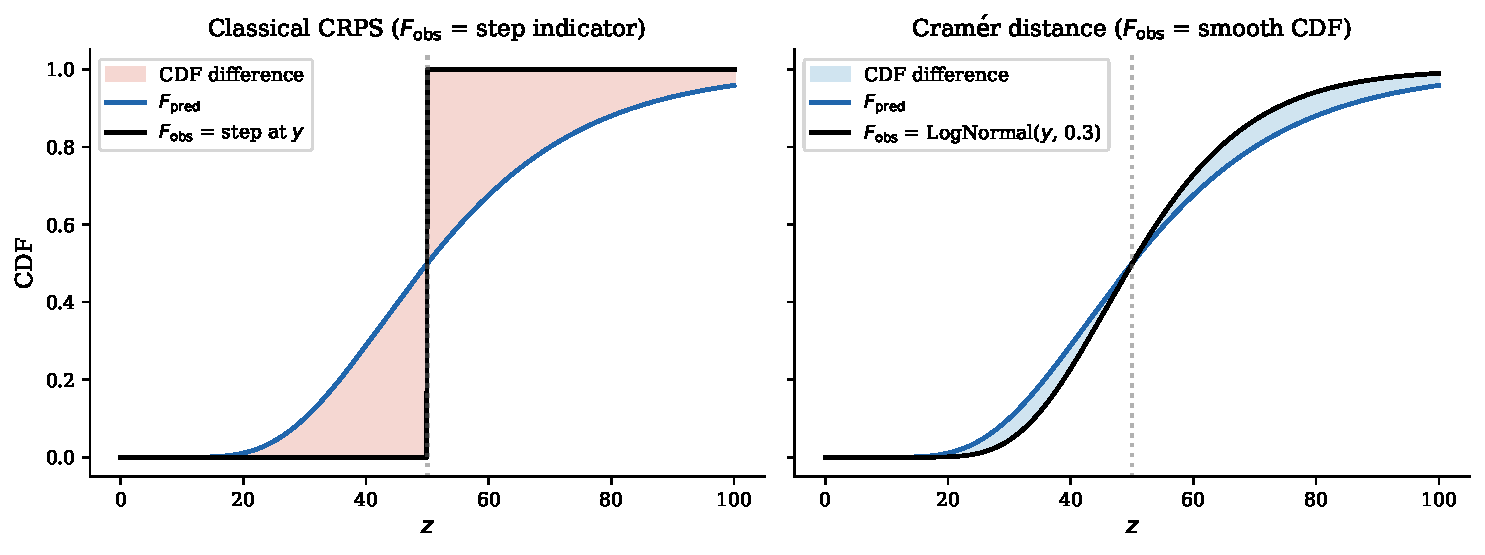
\includegraphics[width=\textwidth]{figures/step_vs_sigmoid.pdf}
    \caption{CDF comparison under two definitions of $F_\text{obs}$. Left: classical CRPS uses a step indicator; the shaded area between the smooth forecast and the hard boundary is large. Right: the Cram\'er-distance reformulation uses a smooth $F_\text{obs}$ reflecting observational uncertainty; a moderately wide forecast is no longer penalised relative to an overconfident one. The shaded region shows the gap $F_\text{pred}(z) - F_\text{obs}(z)$; the Cram\'er-distance integrand is its square.}
    \label{fig:step_vs_sigmoid}
\end{figure}
